\documentclass[Main]{subfiles}

\begin{document}
\chapter{Lagrangian Systems and Pierels Brackets}
   %introduzione
	\danger .. introduzione

	\section{Abstract Lagragian Systems}
	%Definizione deI sistemi Lagrangiani in Astratto
	\danger introduzione
	\begin{definition}[Lagrangian System]
	Pair $(E, \mathcal{L} )$ composed of:
		\begin{itemize}
			\item $E \xrightarrow{\pi} M$ smooth fiber bundle of typical fiber $Q$ called \emph{"configuration bundle"}.
			\item	$ \Lagrangian : J^r E \rightarrow \wedge^m T^*M$ bundle-morphism from the r-th Jet Bundle to  the top-dimensionial forms bundle over the base manifold $M$  called \emph{"Lagrangian density"} or simply \emph{"Lagrangian"} of r-th order.
		\end{itemize}
	\end{definition}	
	
	
	\subsection{Kinematics}
	%Fibrato Configurazione incompassa la cinematica
	The configuration bundle encompass all the kinematical structure of the system, the pivotal role is played by the smooth sections  which are to be understood as all the possible conformation of the system.

	\begin{notationfix}
		\begin{displaymath}
			\Conf \coloneqq \Gamma^\infty(M,E)
		\end{displaymath}
		Space of kinematic configurations.
	\end{notationfix}

	A section is not a statical configuration, equivalent to a specific point in the configuration space of ordinary classical systems, but has to be seen as a specific realization of the kinematics in the sense of  a complete description of a possible motion.
	At this level of abstraction, since no space-time structure has been specified, terms like stasis and motion must be taken with care .The natural physical interpretation should be clearly manifested through the concrete realization of systems with discrete and continuous degree of freedom.
	
	\begin{observation}[Mathematical structure]
	Mathematically speaking this set should be regarded as an infinite dimensional Manifold. 
	
	This framework provides a geometric characterization of the notion of variations as tangent vectors on the the space of kinematic configurations .\cite{Forger2005}
	\end{observation}
	
	\begin{observation}[Coordinate Representation]
	The choice of a chart atlas $\Atlas(M)$ on the base space $M$ and $\Atlas(E)$ on the total space $E$ provides a correspondence between each configuration $\gamma \in \Conf$ and family of smooth real functions $\{f_{\alpha \beta}:A_\alpha \subset \Real^m \rightarrow \Real^q \}$.
	The process is trivial:
	\begin{displaymath}
		\gamma \in \Conf \mapsto \{f_{A,U}=\psi_U \circ \gamma \circ \psi_A^{-1} \vert (A,\psi_A) \in \Atlas(M), (U,\psi_U)\in \Atlas(E)   \}
	\end{displaymath}
	
	%	$\forall (A,\psi_A)$ local chart on $M$ and $(U,\psi_U)$ local chart on $E$ such that $\gamma(A) \cap U \neq \emptyset$ $f_{A,U}=\psi_U \circ \gamma \circ \psi_A^{-1}$

	Since the whole section as a global object is quite difficult to handle is customary in field theory to work in the more practical local representation. 
	\end{observation}	
	
	\begin{observation}[Further specification of the system's kinematics]
	 	The general formalism doesn't require any other structure to be carried forward.
	 	Additional structure on the fiber , the base or the whole bundle are to be prescribed in order to specify a precise physical model, e.g. the spin structure for the Dirac Field.\cite{Benini}
	 \end{observation}	
	
	\begin{figure}[h!]
 	 	\caption{Geometric picture of the basic kinematic structure.}
 	 	\danger immagine
   		%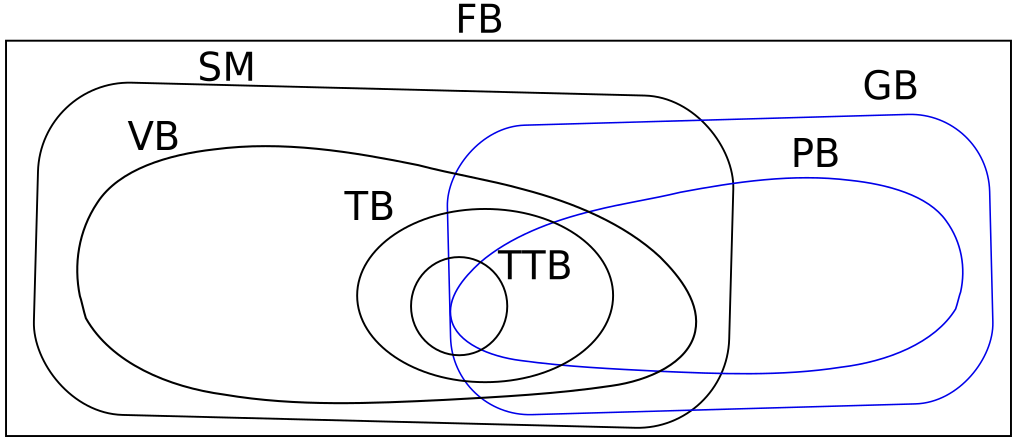
\includegraphics[width=0.5\textwidth]{Pictures/EuleroVenn_Bundles} 
  		\centering
	\end{figure}	
	
	\subsection{Dynamics}
	%la lagrangiana incompassa la dinamica
	The Lagrangian density is the object that contains all the information about the dynamic evolution of the system.
	In fact, when a dynamical principle is provided, $\Lagrangian$ determines univocally a differential operator $P$ on the kinematics configurations space $\Conf$.
	This operator is named  \emph{"equations of motion"} operator and has the role to select the dinamically compatible configuration among all the admissible kinematic configurations of $\Conf$; exactly as it happens in analytical mechanics where the dynamic equations shape the natural motions.
	\begin{notationfix}
		Provided an equations of motion operator
		\begin{displaymath}
			P: \Conf \rightarrow \Conf
		\end{displaymath}
		The space
		\begin{displaymath}
		\Sol \coloneqq \ker(P) \subset \Conf
		\end{displaymath}
		is called \emph{"Space of Dynamical Configurations"}.
	\end{notationfix}
	

	%la classe delle densità lagrangiane
	In order to reconstruct the system's dynamic from the Lagrangian density we have to understand the mathematical nature of $\Lagrangian$.
	$\Lagrangian$ maps point $q_p$ on the fiber $J^r_p E$ to a m-form on $T_p M$.
	Recalling the definition of jet bundles is clear that for each smooth section on $E$ is associated a smooth section on the b$J^rE$ :
	\begin{displaymath}
		\phi \in \Gamma^\infty (E) \mapsto (\phi, \partial_\mu \phi, \partial_{\mu, \nu} \phi , \ldots \partial_{\vec{\alpha}}\phi)
	\end{displaymath}
	where  $\vec{\alpha}$ is a multi-index of length r.
	The correspondence is not univocal since sections equal up to the r-th order define the same jet section.
	The smoothness of $\Lagrangian$ ensure that each jet bundle section is mapped to a smooth section of the top-forms bundle.
	The
		
	\footnote{$\forall p \in M$, $\Lagrangian$ maps the point $q_p$ on the fiber $J^r_p E$ to a n-form on $T_p M$.}

	\begin{definition}[Lagrangian functions on the bundle $E$]
	
	
	\end{definition}
	
	%il funzionale lagrangiana totale e azione
	
	%Principio di minima azione e operatore delle equazioni del moto
	
	%Spazio delle configurazioni di Campo
	
	
	
	\subsection{Generalization}
	%Sistemi evolutivi e sistemi hamiltoniani	
	From the preceding analysis is clear that the central object of the dynamics is 	the operator P \emph{motion equation operator} fa le veci delle equazioni della dinamica
	\begin{definition}[Evolutive System]
	
	\end{definition}
	
%-_-_-_-_-_-_-_-_-_-_-_-_-_-_-_-_-_-_-_-_-_-_-_-_-_-_-_-_-_-_-_-_-_-_-_-_-_-_-_-_-_-_-_-_-_-_-_-_-_-_-_-_-_-_-_
\newpage
	\section{Concrete Realization}
	%esibiamo quanto è ampia la nostra definizione
		\subsection{Fields on curved Background}
		%M è spazio tempo,
		%bundle è lineare per prevedere il principio di sovrapposizione
		%M è glob iper e P è green iper per tener conto del comporatamento propagativo
		\subsection{Finite Degree systems}
		  % il fibrato non è vettoriale
		  % le configurazioni sono curve
		  % 
		
%-_-_-_-_-_-_-_-_-_-_-_-_-_-_-_-_-_-_-_-_-_-_-_-_-_-_-_-_-_-_-_-_-_-_-_-_-_-_-_-_-_-_-_-_-_-_-_-_-_-_-_-_-_-_-_
\newpage
	\section{Geometric mechanics of Finite Degree systems}
	%L'approccio usato generalmente è deduttivo dal particolare al generale
	%parlare di spazio delle fasi, forma simplettica, legendre
	%osservabili classici parentesi di poisson
	
	\subsection{Linear dynamical systems}	
	
%-_-_-_-_-_-_-_-_-_-_-_-_-_-_-_-_-_-_-_-_-_-_-_-_-_-_-_-_-_-_-_-_-_-_-_-_-_-_-_-_-_-_-_-_-_-_-_-_-_-_-_-_-_-_-_
\newpage
	\section{Peierls Brackets}
	%peierels vs poisson (sharan)
	
	\subsection{Finite Dimensional case}
	
%-_-_-_-_-_-_-_-_-_-_-_-_-_-_-_-_-_-_-_-_-_-_-_-_-_-_-_-_-_-_-_-_-_-_-_-_-_-_-_-_-_-_-_-_-_-_-_-_-_-_-_-_-_-_-_
\newpage
	\section{Eliminata}
	\begin{itemize}
		\item quando parlo della cinematica mi piacerebbe dare indicazioni sulla struttura matematica dello spazio delle configurazioni cinematiche:
			\begin{enumerate}
				\item costituisce una frechet manifold ( gli unici risultati che ho trovato sono quelli di Palais di "non linear global analysis"
				\item le curve parametrizzate sono le variazioni
				\item classi di equivalenza definiscono delle variazioni infinitesime che costituiscono lo spazio tangente allo spazio delle configurazioni cinematiche
				\item questo spazio tangente è isomorfo allo spazio delle sezioni del pullback rispetto alla sezione $\phi\in C$ del verical bundle (vedere forger romero)
				\item il problema dell'atlante e della rappresentazione delle sezioni in carta locale ( da scegliere sia sul total space E che sul base space M)
			\end{enumerate}
	\end{itemize}
	
\end{document}